\documentclass[class=ctexart,crop=false]{standalone}

\usepackage{amsmath,amssymb,enumitem,empheq,tkz-euclide,
diagbox,wrapfig,pgfplots,geometry}
%\geometry{a4paper,scale=0.9}
\pgfplotsset{compat=newest}
%\usepgfplotslibrary{external}
%\tikzexternalize
\renewcommand\parallel{\mathrel{/\mskip-2.5mu/}}

\newcommand\px{\mathrel{/\mkern-5mu/}}  %平行
\newcommand\pxeq{\mathrel{\vcenter{     %平行且等于
\ialign{\hfil##\hfil\crcr
$\scriptstyle\px\!$\crcr
\noalign{\nointerlineskip\vskip1pt}$=$\crcr}}}}

%\setCJKmainfont{SimSun}       %设置西文字体为times new roman
%\setCJKsansfont{SimSun}             %设置中文字体为宋体
%\setCJKmonofont{STKaiti}
%\setsansfont{TeX Gyre Termes}            %设置typewriter family中文字体为楷体
%\setmonofont{TeX Gyre Termes}

\usetikzlibrary{calc,intersections,through,backgrounds,patterns}
\newcounter{para}
\newcommand\mypara{\par\refstepcounter{para}\thepara.\space}%设置typewriter family西文字体为times new roman
\newcommand*\circled[1]{\tikz[baseline=(char.base)]{
            \node[shape=circle,draw,inner sep=1pt] (char) {#1};}}

\newcommand{\rnum}[1]{\romannumeral #1}
\newcommand{\RNum}[1]{\uppercase\expandafter{\romannumeral #1\relax}}
\begin{document}
梯形 $PQCB$ 中, $PQ \parallel BC$,延长 $CQ,BP$ 相交与 $A$.连接 $PC,QB$ 交于 $O$,连接 $AO$ 并延长,交 $BC$ 于 $D$.\\
求证 $D$ 为 $BC$ 中点.\hfill\hphantom\quad
    \begin{wrapfigure}{r}{0.3\textwidth}
    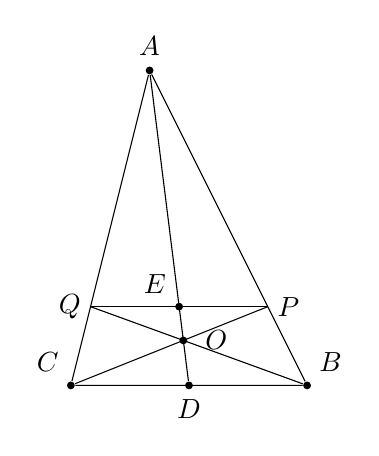
\begin{tikzpicture}
        \node[label={[label distance=0.005cm]90:{$A$}},circle,fill,inner sep=1pt] (A) at (0,4) {};
        \node[label={[label distance=0.005cm]60:{$B$}},circle,fill,inner sep=1pt] (B) at (2,0) {};
        \node[label={[label distance=0.005cm]120:{$C$}},circle,fill,inner sep=1pt] (C) at (-1,0) {};
        \path[name path=lPQ] (-1,1)--(2,1);
        \draw[name path=triABC] (A)--(B)--(C)--(A);
        \path[name intersections={of = lPQ and triABC,
        by={[label=right:$P$]P,[label=left:$Q$]Q}}];
        \draw[name path=QB] (Q)--(B);
        \draw[] (P)--(Q);
        \draw[name path=PC] (P)--(C);
        \path[name intersections={of= PC and QB,by=O}];
        \node[label={[label distance=0.1cm]0:{$O$}},circle,fill,inner sep=1pt]  at (O){};
        \node[label={[label distance=0.005cm]270:{$D$}},circle,fill,inner sep=1pt] (D) at ($(B)!.5!(C)$){};
        \draw[name path=lAD] (A)--(D);
        \path[name intersections={of=lPQ and lAD,by=E}];
        \node[label={[label distance=0.005cm]135:{$E$}},circle,fill,inner sep=1pt]  at (E){};
    \end{tikzpicture}
\end{wrapfigure}
解:\\
易知 $\triangle APQ \sim \triangle ABC$\\
故设 $\frac{\overrightarrow{AQ}}{\overrightarrow{AC}}
=\frac{\overrightarrow{AP}}{\overrightarrow{AB}}=\frac{\overrightarrow{PQ}}{\overrightarrow{BC}}=\lambda$\\
则 $\overrightarrow{QC}=(1-n)\overrightarrow{AC}$,\\
同时$\triangle OPQ\sim\triangle OCB,
\triangle OEP\sim\triangle ODC$\\
则 $\frac{\overrightarrow{OE}}{\overrightarrow{OD}}
=\frac{\overrightarrow{OP}}{\overrightarrow{OC}}
=\frac{\overrightarrow{QP}}{\overrightarrow{BC}}=\lambda$ \\
$\begin{aligned}[t]
     \overrightarrow{PO}&=\lambda\overrightarrow{OC}\\
     \overrightarrow{PC}&=(1+\lambda)\overrightarrow{OC}\\
     \overrightarrow{OC}&=\frac{\overrightarrow{PB}+\overrightarrow{BC}}{1+\lambda}\\
     &=\frac{(1-\lambda)\overrightarrow{AB}+\overrightarrow{AC}-\overrightarrow{AB}}{1+\lambda}\\
     &=\frac{\overrightarrow{AC}-\lambda\overrightarrow{AB}}{1+\lambda}\\
     \overrightarrow{AO}&=\overrightarrow{AC}-\overrightarrow{OC}\\
     &=\frac{\lambda\overrightarrow{AC}+\lambda\overrightarrow{AB}}{1+\lambda}\\
     &=\frac{\lambda}{1+\lambda}(\overrightarrow{AB}+\overrightarrow{AC})\\
\end{aligned}$\\
故有 $\mu,\nu$使得 $\begin{aligned}[t]
    \overrightarrow{AD}&=(\frac{\mu\lambda}{1+\lambda})(\overrightarrow{AB}+\overrightarrow{AC})\\
    &=\nu\overrightarrow{AB}+(1-\nu)\overrightarrow{AC}
\end{aligned}$\\
解得 $\nu=\frac{1}{2}$, 故 $D$ 为 $BC$ 中点.
\end{document}